\documentclass[a4paper]{article}
%\usepackage{geometry}

% if you need to pass options to natbib, use, e.g.:
%     \PassOptionsToPackage{numbers, compress}{natbib}
% before loading neurips_2018

% ready for submission
% \usepackage{neurips_2018}

% to compile a preprint version, e.g., for submission to arXiv, add add the
% [preprint] option:
%     \usepackage[preprint]{neurips_2018}

% to compile a camera-ready version, add the [final] option, e.g.:
     \usepackage[final]{nips_2018}

% to avoid loading the natbib package, add option nonatbib:
%     \usepackage[nonatbib]{neurips_2018}

\usepackage[utf8]{inputenc} % allow utf-8 input
\usepackage[T1]{fontenc}    % use 8-bit T1 fonts
\usepackage{hyperref}       % hyperlinks
\usepackage{url}            % simple URL typesetting
\usepackage{booktabs}       % professional-quality tables
\usepackage{amsfonts}       % blackboard math symbols
\usepackage{nicefrac}       % compact symbols for 1/2, etc.
\usepackage{microtype}      % microtypography

\usepackage{graphicx}
\usepackage{subcaption}
\usepackage{hyperref}
\usepackage{amsmath}
\DeclareMathOperator*{\argmax}{argmax}
\DeclareMathOperator*{\argmin}{argmin}
\usepackage{algorithm}
\usepackage{algpseudocode}
\usepackage{enumerate}
\usepackage[numbered]{bookmark}


\title{Advanced Topics on Robotics \\ Homework 2}

% The \author macro works with any number of authors. There are two commands
% used to separate the names and addresses of multiple authors: \And and \AND.
%
% Using \And between authors leaves it to LaTeX to determine where to break the
% lines. Using \AND forces a line break at that point. So, if LaTeX puts 3 of 4
% authors names on the first line, and the last on the second line, try using
% \AND instead of \And before the third author name.

\author{%
  Alexandre M.~F.~Dias\\%\thanks{Use footnote for providing further information
    %about author (webpage, alternative address)---\emph{not} for acknowledging
    %funding agencies.} \\
  Department of Electrical and Computer Engineering\\
  Instituto Superior Técnico - University of Lisbon\\
  \texttt{alexandre.f.dias@tecnico.ulisboa.pt} \\
  % examples of more authors
  % \And
  % Coauthor \\
  % Affiliation \\
  % Address \\
  % \texttt{email} \\
  % \AND
  % Coauthor \\
  % Affiliation \\
  % Address \\
  % \texttt{email} \\
  % \And
  % Coauthor \\
  % Affiliation \\
  % Address \\
  % \texttt{email} \\
  % \And
  % Coauthor \\
  % Affiliation \\
  % Address \\
  % \texttt{email} \\
}

\begin{document}
% \nipsfinalcopy is no longer used

\maketitle

%\begin{abstract}
%  The abstract paragraph should be indented \nicefrac{1}{2}~inch (3~picas) on
%  both the left- and right-hand margins. Use 10~point type, with a vertical
%  spacing (leading) of 11~points.  The word \textbf{Abstract} must be centered,
%  bold, and in point size 12. Two line spaces precede the abstract. The abstract
%  must be limited to one paragraph.
%\end{abstract}

\section{Introduction}


% finite MDPs: check Chapter 3 of RL book [\cite{10.5555/3312046}]
The problem at hand is a finite Markov Decision Process (finite MDP), as the state, action and reward sets are finite sets. In Fig. \ref{fig:problem}, the problem is illustrated, according to \cite{LITTMAN1995362}. It consists of 60 states, which correspond to the 4 possible orientations (north, south, west, and east) in each of the 15 rooms. One of the rooms (room 15) corresponds to the 4 goal states (states 57 to 60) and 4 of the rooms contain landmarks (visible to the robot when facing south in a room north of a landmark room). There are 5 possible actions in each room (stay in place, move forward, turn right, turn left, turn around). There are also 21 observations, which correspond to i) each possible combination of the presence of a wall in each of the 4 orientations, ii) the four landmarks and iii) reaching each of the 4 goal states.

% Tabular methods definition: from page 23
Tabular solution methods are those where the state and action spaces are small enough so that value functions can be represented as arrays or tables. In this homework, three tabular solution methods for solving finite MDPs are explored. The first two, Policy Iteration and Value Iteration, are Dynamic Programming (DP) methods and on-policy methods, while the other one, Q-learning, is a Temporal-Difference (TD) method and an off-policy method. DP methods require a complete model of the environment (they are model based), while TD methods require no model (they are model free). Although Policy Iteration was not required to be experimented with, it is explored as its results provide a baseline to the other methods (optimal policy and optimal value function). Under certain conditions, all of these methods are guaranteed to converge to the optimal solution, i.e., the value function converges to the optimal value function, with the corresponding policy or policies being optimal\footnote{A value function may correspond to one policy or several distinct policies, and in the same way an optimal value function may correspond to one optimal policy or several distinct optimal policies.}.

\begin{figure}[htbp]
\centering
%\includegraphics[width=\linewidth]{problem_60_states.png}
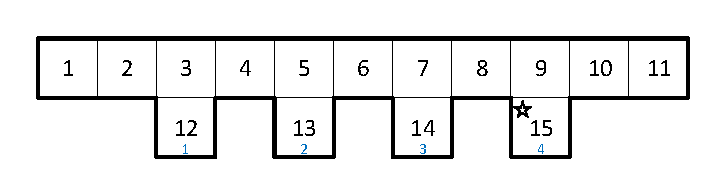
\includegraphics[width=\linewidth]{figures/problem.pdf}
\caption{The problem at hand: 60 states, corresponding to 15 rooms in which the robot can have 4 possible orientations (facing north, south, west and east); the room marked with a star corresponds to the 4 goal states (states 57 to 60) and the rooms numbered from 1 to 4, in blue, contain a landmark each.}
\label{fig:problem}
\end{figure}

\section{Full observability: Value Iteration}

The update operation performed in Value Iteration combines a \textit{truncated} Policy Evaluation --- a single sweep through all non-goal states $s \in \cal{S}$ --- and Policy Improvement:

\begin{align}
v_{k+1}\left( s \right) = \max_{a} \sum\limits_{s',r} { p\left( {s',r|s,a} \right) \left[ r + \gamma v_{k}\left( s' \right) \right] }, \forall s \in {\cal S}, \forall s' \in {\cal S}^{+}.
\end{align}

For details on Policy Evaluation, Policy Improvement and the Policy Iteration algorithm the reader is referred to Section \ref{app_sec:policy_iteration} of the appendix. Sequence $\left\{ v_k \right\}$ can be shown to converge to $v_{*}$ under the same conditions that guarantee the existence of $v_{*}$ (either $\gamma < 1$ or termination is guaranteed from all states).

The Value Iteration algorithm is implemented according to Algorithm \ref{alg:value_iteration}, which is a slightly modified version of that in Section 4.4 of \cite{10.5555/3312046} --- similarly to Policy Iteration (Algorithm \ref{alg:policy_iteration}), it also uses the relative change in the value function norm as convergence criterion instead of the maximum absolute component change of the value function.

In Fig. \ref{fig:value_iteration}, the results of running Value Iteration are shown. The upper chart of Fig. \ref{fig:value_iteration} depicts the policy difference\footnote{For details on the policy difference evaluation metric, see Section \ref{app_sec:policy_difference} of the Appendix} between the policy corresponding to current value function in Value Iteration and the optimal policy previously determined in Policy Iteration (Table \ref{tab:optimal_policy}).

The middle chart of Fig. \ref{fig:value_iteration} depicts the evolution of the relative change in the value function norm (convergence criterion). When comparing both upper and middle charts of Fig. \ref{fig:value_iteration}, one can easily observe that the policy underlying the value function converges to the optimal policy much earlier than the value function is considered to have converged to the optimal value function --- the policy is already optimal after 9 iterations, with the convergence criterion being of the order of 10\textsuperscript{-2}, while convergence of the value function is only attained after 43 iterations ($\theta = 10^{-6}$).

The lower chart of Fig. \ref{fig:value_iteration} shows how the value function evolves throughout iterations for each state. One can observe that the value function does not increase monotonically for each state as the algorithm is executed. The reason for this is that a \textit{truncated} rather than \textit{full} Policy Evaluation --- as in the Policy \textit{Iteration} algorithm --- is employed. On the other hand, the value function converges to the optimal value function, which can be verified by comparing the line corresponding to the last iteration (iteration 43) with Fig. \ref{fig:policy_iteration}.

\begin{figure}[htbp]
\centering
\includegraphics[width=\linewidth]{plots/plot_value_iteration.pdf}
\caption{Policy difference $\Delta \pi$, relative change in the value function norm (convergence criterion) and state value function $V(s)$ for the execution of the Value Iteration algorithm ($\theta=10^{-6}$).}
\label{fig:value_iteration}
\end{figure}


\section{Full observability: Q-learning}

Two sets of experiments were carried out to explore the Q-learning algorithm. The first set of experiments consisted in trying values for $\alpha_n$ and $\varepsilon$ such that convergence was ensured, while in the second set of experiments there was no convergence guarantee, although convergence could still be attained through proper choice of values for $\alpha_n$ and $\varepsilon$. In the Q-learning algorithm, the update rule is

\begin{align*}
%\label{eq:policy_difference_explained4}
Q(s,a) \gets Q(s,a) + \alpha_n \left[ {r + \gamma \max_{a} Q(s',a) - Q(s,a)} \right]
\end{align*}

% I am not sure about these convergence criteria (RL book vs ATR slides vs Stack Overflow) 
% https://stackoverflow.com/questions/59709726/criteria-for-convergence-in-q-learning
To ensure convergence, it is required that all state-action pairs continue to be updated, i.e., in the limit (infinite algorithm steps) each state-action pair is taken an infinite number of times; it is also required that the sequence of step-size values $\alpha_n$ fulfills two conditions:

\begin{align}
%\label{eq:policy_difference_explained4}
\sum\limits_{n=1}^{\infty} \alpha_{n} = \infty \label{eq:convergence_criterion_sum}\\ 
\sum\limits_{n=1}^{\infty} \alpha_{n}^{2} < \infty \label{eq:convergence_criterion_sum_squared}
\end{align}

According to these conditions, in the first set of experiments\footnote{Although conditions (\ref{eq:convergence_criterion_sum}) and (\ref{eq:convergence_criterion_sum_squared}) refer to \textit{each} state-action pair, in the simulations carried out $\alpha_n = \alpha / n$ refers to the \textit{overall} total number of steps, not to the total number of steps of a \textit{particular} state-action pair; this still ensures that both conditions are met and has proved in simulations to converge \textit{faster} to the true state-action value function $Q(s,a)$ and for a \textit{broader} range of values for $\alpha$ and $\varepsilon$.} $\alpha_n = \alpha / n$ for some $\alpha > 0$, in order to ensure convergence,  and $\varepsilon > 0$ to ensure that each state-action pair is, in the limit, taken an infinite number of times. In the second set of experiments, $\alpha_n = \alpha$, for some $\alpha > 0$, thus convergence is not ensured as condition (\ref{eq:convergence_criterion_sum_squared}) is not fulfilled.

In Fig. \ref{fig:hyperparams_convergence}, the two tables summarize the number of episodes (upper cell value) and total number of steps (lower cell value) necessary until convergence to the optimal \textit{policy}, for distinct combinations of values for $\alpha$ and $\varepsilon$ in each of the two sets of experiments. The number of steps needed until convergence is considered a proxy for the computational effort required. In Fig. \ref{fig:hyperparams_convergence}.(\subref{fig:table_results_convergence_not_ensured}), the designation \textit{oscill.} conveys that, although the optimal policy is attained, during the remainder of the algorithm execution the policy underlying the state-action value function $Q(s,a)$ \textit{oscillates} between the optimal policy and non-optimal policies. 

% Note that convergence here refers to the policy corresponding to the state-action value function $Q(s,a)$ converging to the optimal policy, not to the state-action value function being optimal.

\begin{figure}[htbp]
%\centering
\begin{subfigure}{\textwidth}
\centering
\includegraphics[scale=0.8]{figures/table_results_convergence_ensured.png}
%\includegraphics[width=\linewidth]{plots/table_results_convergence_ensured.png}
\caption{Convergence ensured}
\label{fig:table_results_convergence_ensured}
\end{subfigure}
\begin{subfigure}{\textwidth}
\centering
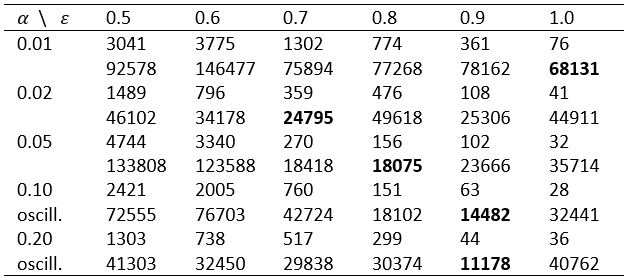
\includegraphics[scale=0.8]{figures/table_results_convergence_not_ensured.png}
\caption{Convergence not ensured}
\label{fig:table_results_convergence_not_ensured}
\end{subfigure}
\caption{Number of episodes (upper cell value) and number of steps (lower cell value) necessary for convergence to the optimal policy, for distinct combinations of hyperparameter values in the two sets of experiments.}
\label{fig:hyperparams_convergence}
\end{figure}

In Figs. \ref{fig:q_learning_convergence_ensured} and \ref{fig:q_learning_convergence_not_ensured}, the evolution of the Q-learning algorithm is illustrated for a set of values achieving the optimal policy within a relatively low total number of steps in each of the sets of experiments (convergence ensured and convergence not ensured, respectively). In the figures, the policy difference, the root mean squared error (RMSE) of the norm difference between $Q(s,a)$ and $Q_{*}(s,a)$ (averaged over states), the relative change in the norm of $Q(s,a)$ and the number of steps in each episode are shown.

Similarly to the Value Iteration algorithm, it can be observed in both Figs. \ref{fig:q_learning_convergence_ensured} and \ref{fig:q_learning_convergence_not_ensured} that in the Q-learning algorithm the value function (now the state-action value function, instead of the state value function) also takes much longer to converge than what is required for the policy underlying the value function to converge to the optimal policy. This is a downside of Q-learning: although convergence to the optimal value function can be ensured, the computation to achieve so is too expensive --- one possibility is to rely on the stabilization of the change in the state-action value function, as shown in both figures, and even then care must be taken (such a metric oscillates by over one order of magnitude).

%It can also be observed that, after a certain number of steps, in the situation where convergence is not ensured (Fig. \ref{fig:q_learning_convergence_not_ensured}) the relative change of the norm of $Q(s,a)$ stabilizes and does not keep decreasing as it is desired.

% --- for instance, in Fig. \ref{fig:q_learning_convergence_ensured}, if we consider that convergence is attained when the relative change in the norm of $Q(s,a)$ is below 10\textsuperscript{-5}, then the required number of steps is about ten thousand or, on average, of the order of 10\textsuperscript{2} per state and of the order of 10\textsuperscript{1} per state-action pair.

In both sets of experiments, Q-learning benefits greatly from exploration in the problem at hand, as convergence is more quickly achieved with relatively high values of $\varepsilon$ (greater or equal than 0.5). Moreover, even a completely random choice of actions ($\varepsilon=1.0$) for the update of $Q(s,a)$ allows achieving convergence within a reasonable total number of steps. This shows that it is very important that each state-action pair keeps being visited as the algorithm executes and not just the state-action pairs considered optimal.


\section{Partial observability: point-based Value Iteration}

In this section, the problem at hand is solved in the POMDP framework, i.e., instead of assuming full state observability as before, partial observability is considered, with observations being used to update belief states (probability distributions over the set of possible states). Therefore, additionally to the uncertainty associated with action outcome (transition model), there is now also uncertainty associated with observation of the state (observation model).

In POMDPs, the (optimal) value function is piecewise linear and convex. Exact value iteration algorithms for POMDPs exist, however the computation of exact solutions for POMDPs is, in general, an intractable problem. For this reason, approximate solution techniques using a sample set of points from the belief space have been devised. Perseus is a randomized point-based approximate value iteration algorithm for solving POMDPs. The algorithm allows approximating the value function with a relatively small number of vectors (relative to the size of the belief points set).

In Table \ref{tab:pomdp_perseus_results}, the results of running the Perseus algorithm and sampling statistics for different belief points set sizes are summarized. In Fig. \ref{fig:pomdp_perseus_results}, further results of the Perseus algorithm execution and sampling statistics for different belief points set sizes are illustrated. In the upper chart, the state value function approximation, computed as the mean\footnote{The reason for this is the state value function being defined as an expectation, and therefore the mean is an estimate of the expectation.} of the cumulative reward over all the simulation runs per non-goal state, is depicted. The lower chart conveys how the algorithm time complexity varies with the size of the belief points set.

The upper chart of Fig. \ref{fig:pomdp_perseus_results} indicates that even a fairly small belief points set size of $| {\cal B} |=100$ already provides a very good approximation of the value function $V(s)$, with the number of vectors defining such approximation being relatively small ($| V |=36$), while also showing that a size of $| {\cal B} |=10$ is clearly insufficient to attain a good approximation. Naturally, since in the POMDP setting the state is not fully observable and the agent must rely on observations, the value of each state can never exceed that of the MDP setting, and in the problem at hand is typically quite lower than the value in the fully observability case.

Regarding algorithmic complexity, Table~\ref{tab:pomdp_perseus_results} shows that the number of approximating vectors is typically one order of magnitude below that of the belief points set size. The lower chart of Fig.~\ref{fig:pomdp_perseus_results} conveys that an increase of one order of magnitude in the belief points set size translates into a increase of less than one order of magnitude (0.60 to 0.70, in $\log_{10}$ scale) in algorithm execution time, showing that, timewise, the algorithm scales well with the belief points set size.

\begin{table}[htbp]
\centering
\begin{tabular}{ r r r r r }
\hline
\multicolumn{1}{c}{\begin{tabular}[c]{@{}c@{}}Belief points\\ set size, $\log_{10}| {\cal B} |$ \\ \end{tabular}} & \multicolumn{1}{c}{\begin{tabular}[c]{@{}c@{}}Value function\\ vector set size, $| V |$ \\ \end{tabular}} & \multicolumn{1}{c}{Iterations} & \multicolumn{1}{c}{\begin{tabular}[c]{@{}c@{}}Value\\ iteration \\ time (s)\end{tabular}} & \multicolumn{1}{c}{\begin{tabular}[c]{@{}c@{}}Success rate\\ \\ (\%)\end{tabular}} \\ \hline
1       &     9 & 30 & 4  & 73 \\
2     &   36 & 72 & 13   & 100 \\
3   & 192 & 94 & 53   & 100 \\
4 & 706 & 94 & 259 & 100 \\ \hline
\end{tabular}
\caption{Execution results of the Perseus algorithm and sampling statistics for different belief points set sizes (convergence criterion of 10\textsuperscript{-3}). The sampling leading to the success rate and discounted cumulative reward metrics was carried out over 1000 runs for each of the 56 non-goal states as start state.}
\label{tab:pomdp_perseus_results}
\end{table}

\begin{figure}[htbp]
\centering
\includegraphics[width=\linewidth]{plots/plot_value_iteration_POMDP.pdf}
\caption{Execution results of the Perseus algorithm and sampling statistics for different belief points set sizes (convergence criterion of 10\textsuperscript{-3}): value function approximation (mean of the cumulative reward over 1000 runs) and algorithm execution time.}
\label{fig:pomdp_perseus_results}
\end{figure}


\section{Conclusions}

In this homework, experimentations considering full and partial observability in the problem at hand were carried out.

For full observability, the Value Iteration algorithm learned the optimal policy and converged to the optimal value function through backup operations, resorting to the transition model. The Q-learning algorithm learned the optimal policy through experimentation (simulated state transitions), without knowledge of the transition model itself. In Q-learning, there is a clear interplay between the step size $\alpha$ and the amount of exploration provided by the $\varepsilon$-greedy policy behavior in the attainment of the optimal policy. Also, even if convergence is not ensured by the values taken by the step size, convergence can still be achieved. 

For partial observability, the Perseus randomized point-based approximate value iteration algorithm was able to attain successful policies with relatively low computational effort, even lower than that of the tabular methods, proving the merit of approximate methods for the value function based on a sample set of the belief space.


\begin{figure}[htbp]
\centering
\includegraphics[width=\linewidth]{plots/plot_Qlearning_a=200.00_e=0.80_min=0.00_episodes_50000.pdf}
\caption{Policy difference $\Delta \pi$, RMSE error of the state-action value function $Q(s,a)$ relative to the optimal state-action value function $Q_{*}(s,a)$, relative change in the state-action value function norm and number of steps required to reach a terminal state in each episode. The hyperparameters $\alpha$ and $\varepsilon$ take values of 1000 and 0.8, respectively, with $\alpha_n = \alpha / n$, where $n$ is the total number of steps so far.}
\label{fig:q_learning_convergence_ensured}
\end{figure}

\begin{figure}[htbp]
\centering
\includegraphics[width=\linewidth]{plots/plot_Qlearning_a=0.02_e=0.70_min=0.00_episodes_50000.pdf}
\caption{Policy difference $\Delta \pi$, RMSE error of the state-action value function $Q(s,a)$ relative to the optimal state-action value function $Q_{*}(s,a)$, relative change in the state-action value function norm and number of steps required to reach a terminal state in each episode. The hyperparameters $\alpha$ and $\varepsilon$ take values of 0.02 and 0.7, respectively, with $\alpha_n = \alpha$.}
\label{fig:q_learning_convergence_not_ensured}
\end{figure}

% falta runtime nas tabelas da Figura 3, Q RMSE and Q norm chng

%https://www.google.com/search?q=initial+values+%22value+iteration%22+minimum
%initialization: value iteration, q-learning
%initialization vs convergence

% discount factor:
% gamma<=1: action 1 is never selected, except in Policy Iteration (special case); 
% gamma > 1: action 1 would always be selected
% important: reward only in the terminal states

% LaTeX formatting:
% 1) table column names
% 2) uniformize references 
\vfill
\newpage
\appendix

\section{Policy Iteration}
\label{app_sec:policy_iteration}

The optimal state value function $v_{*}$ satisfies the Bellman optimality equation, 

\begin{align}
v^{*}\left( s \right) &= \max_{a} \mathbb{E} \left[ G_t | S_t =s, A_t = a \right] \\
                              &= \max_{a} \mathbb{E} \left[ R_{t+1} + \gamma v^{*}\left( S_{t+1} \right) | S_t = s, A_t = a \right] \\
                              &= \max_{a} \sum\limits_{s',r} { p\left( {s',r|s,a} \right) \left[ r + \gamma v^{*}\left( s' \right) \right] },
\end{align}

$\forall s \in \cal{S}$, $\forall s' \in \cal{S^{+}}$, $\forall a \in \cal{A}$, and by convention $v(s'') = 0, s'' \in \cal{S^{+}} \setminus \cal{S}$ ($s''$ is a terminal or goal state).

If a policy $\pi$ is being followed, the \textit{state value function for policy} $\pi$ is given by:

\begin{align}
v^{\pi}\left( s \right) &= \mathbb{E}^{\pi} \left[ G_t | S_t =s \right] \\
                              &= \mathbb{E}^{\pi} \left[ R_{t+1} + \gamma v^{\pi}\left( S_{t+1} \right) | S_t = s \right] \\
                              &= \sum\limits_{a}^{|{\cal A}|} \pi \left( a|s\right) \sum\limits_{s',r} { p\left( {s',r|s,a} \right) \left[ r + \gamma v^{\pi}\left( s' \right) \right] },
\end{align}

% existence and uniqueness: Section 4.1 Policy Evaluation (Prediction), page 74
where $\pi \left( a | s \right)$ is the \textit{probability} of taking action $a$ in state $s$ under policy $\pi$. The existence and uniqueness of $v^{\pi}$ is guaranteed if either $\gamma < 1$ or termination is guaranteed from all states under policy $\pi$. The associated update rule is 

\begin{align}
v_{k+1}\left( s \right) = \sum\limits_{a}^{|{\cal A}|} \pi \left( a|s\right) \sum\limits_{s',r} { p\left( {s',r|s,a} \right) \left[ r + \gamma v_{k}\left( s' \right) \right] },
\end{align}

which converges to $v^{\pi}$ as $k \to \infty$, and this algorithm is called \textit{iterative} policy evaluation. The value function updates for each state $s$ can be performed in place, with the updated values being immediately available, or only be available after $v_{k+1}\left( s \right)$ has been computed for all $s \in \cal{S}$. In Policy Evaluation, the estimated value function $v(s)$ is updated for a policy $\pi \left( s \right)$ and for each non-terminal state, until convergence --- this is also known as the \textit{prediction} problem.

In Policy Improvement, given the state value function for a given policy, $v^{\pi}$, one intends to find a new policy $\pi'$ such that $v_{\pi'}\left( s \right) \geq v_{\pi}\left( s \right)$, $\forall s \in \cal{S}$, and if the inequality is strict for at least one state $s \in \cal{S}$, then policy $\pi'$ is better than policy $\pi$. Policy Improvement yields a policy $\pi'$ that is strictly better than policy $\pi$, unless policy $\pi$ is already optimal. The new policy $\pi'$ is obtained through

\begin{align}
\pi'\left( s \right) &= \argmax_{a} q^{\pi} \left( s,a \right) \\
                         &= \argmax_{a} \mathbb{E} \left[ R_{t+1} + \gamma v^{\pi}\left( S_{t+1} \right) | S_t = s , A_t = a \right] \\
                         &= \argmax_{a} \sum\limits_{s',r} { p\left( {s',r|s,a} \right) \left[ r + \gamma v^{\pi}\left( s' \right) \right] },
\end{align}

$\forall s \in \cal{S}$, $\forall s' \in \cal{S^{+}}$.

The Policy \textit{Iteration} method consists in alternating between Policy Evaluation and Policy Improvement until convergence to the optimal policy and corresponding optimal value function. Policy Iteration execution is outlined in Algorithm \ref{alg:policy_iteration}. Algorithm \ref{alg:policy_iteration} is a slightly modified version of that in Section 4.3 of \cite{10.5555/3312046}, in that it

\begin{enumerate}[i.]
\item uses the relative change in the value function norm as convergence criterion instead of the maximum absolute component change of the value function --- this makes the convergence criterion sensitive to small absolute changes that are significant in relative terms, e.g., when a relatively great number of steps is required to achieve a reward only in a terminal state and/or the discount factor is relatively small 
\item considers an equiprobability apportioning scheme --- all optimal actions for a given state are assigned equal probability; this works for both stochastic and deterministic policies (the latter being the case in the problem at hand), as the value function for a given policy is determined \textit{in expectation}, i.e., assigning probability 1 to a single optimal action (deterministic) leads to the same result, in expectation, as assigning probability $1/N$ to $N$ optimal actions (stochastisc or deterministic with more than one optimal action for a given state)
\end{enumerate}

Moreover, the algorithm performs in-place updates (in line \ref{alg:policy_iteration_inplace}, $V(s')$ is used, which is eventually an already updated value of the value function for state $s'$). However, the code implementation does not perform in-place updates; it does, nonetheless, perform vectorized operations, which are still faster than carrying out updates for each individual state $s \in {\cal S}$. 

In Fig. \ref{fig:policy_iteration} and Table \ref{tab:optimal_policy}, the results of running Policy Iteration are shown --- respectively, the optimal value function for the non-terminal states and the optimal action in each state (optimal policy).

Important: explain why action 1 (stay in the same state) is never selected

\begin{figure}[htbp]
\centering
\includegraphics[width=\linewidth]{plots/plot_policy_iteration.pdf}
\caption{Optimal state value function $v(s)$ after the execution of the Policy Iteration algorithm ($\theta=10^{-6}$).}
\label{fig:policy_iteration}
\end{figure}

\begin{table}[htbp]
\centering
\begin{tabular}{| p{1cm} | c c c c c |} 
 \hline
 room & 1 & 2 & 3 & 4 & 5 \\ %[0.5ex] 
 state & 1 2 3 4 & 5 6 7 8 & 9 10 11 12 & 13 14 15 16 & 17 18 19 20 \\
 \hline
 optimal action & 3 2 5 4 & 3 2 5 4 & 3 2 5 4 & 3 2 5 4 & 3 2 5 4 \\ 
 \hline\hline
 room & 6 & 7 & 8 & 9 & 10 \\ %[0.5ex] 
 state & 21 22 23 24 & 25 26 27 28 & 29 30 31 32 & 33 34 35 36 & 37 38 39 40 \\ %[0.5ex] 
 \hline
 optimal action & 3 2 5 4 & 3 2 5 4 & 3 2 5 4 & 4 3 2 5 & 5 4 3 2 \\ [1ex]
 \hline\hline
 room & 11 & 12 & 13 & 14 & 15\\ %[0.5ex] 
 state & 41 42 43 44 & 45 46 47 48 & 49 50 51 52 & 53 54 55 56 & 57 58 59 60\\ %[0.5ex] 
 \hline
 optimal action & 5 4 3 2 & 2 5 4 3 & 2 5 4 3 & 2 5 4 3 & - - - -\\ [1ex]
 \hline
\end{tabular}
\caption{Optimal policy for the problem at hand. In each room, each state corresponds to one of the four possible orientations (north, south, west, and east) and there are five possible actions (stay in place, move forward, turn right, turn left, turn around) in each state.}
\label{tab:optimal_policy}
\end{table}


\vfill
\newpage
\section{Policy difference}
\label{app_sec:policy_difference}
The policy difference between policy $\pi_1$ and policy $\pi_2$, $\Delta \pi$, is defined as the norm\footnote{\url{https://en.wikipedia.org/wiki/Matrix_norm}}:

\begin{align}
\label{eq:policy_difference}
\Delta \pi  = \frac{1}{2}  \left\| {\pi_{1} (s,a) - \pi_{2} (s,a)} \right\|_{1,1} = \frac{1}{2}  \sum\limits_{i}^{|{\cal S}|} \sum\limits_{j}^{|{\cal A}|} {\left| \pi_{1} (s_i, a_j) - \pi_{2} (s_i, a_j) \right|}
\end{align}

The intuition behind (\ref{eq:policy_difference}) is that, if for a certain state $s_i$ the \textit{only} optimal action $a'$ to be taken according to policy $\pi_1$ is different from the \textit{only} optimal action $a''$ to be taken according to policy $\pi_2$, then

\begin{align*}
\label{eq:policy_difference_explained1}
\frac{1}{2} \sum\limits_{j}^{|{\cal A}|} {\left| \pi_{1} (s_i, a_j) - \pi_{2} (s_i, a_j) \right|} &= \frac{1}{2} \left( \left| \pi_{1} (s_i, a') - \pi_{2} (s_i, a') \right| + \left| \pi_{1} (s_i, a'') - \pi_{2} (s_i, a'') \right| \right) \\ &= \frac{1}{2} \left(1 + 1\right) = 1
\end{align*}

since

\begin{align*}
%\label{eq:policy_difference_explained2}
& \left| \pi_{1} (s_i, a_j) - \pi_{2} (s_i, a_j) \right| = \left| 1 - 0 \right| = 1 \vee \left| \pi_{1} (s_i, a_j) - \pi_{2} (s_i, a_j) \right| = \left| 0 - 1 \right| = 1, \\
& a_j = a' \vee a_j = a'',
\end{align*}

and

\begin{align*}
%\label{eq:policy_difference_explained4}
& \left| \pi_{1} (s_i, a_j) - \pi_{2} (s_i, a_j) \right| = \left| 0 - 0 \right| = 0, \\
& a_j \ne a' \wedge a_j \ne a''. 
\end{align*}

In short, for deterministic policies where $\pi (s_i,a_j) = 1$ or $\pi (s_i,a_j) = 0$, $\forall s_i \in {\cal S}$, $\forall a_j \in {\cal A}$, which is the case in the problem at hand, the policy difference $\Delta \pi$ is equal to the number of states for which the action to be taken according to policy $\pi_{1}$ differs from the action to be taken according to policy $\pi_{2}$.


\vfill
\newpage
\section{Algorithms}

\begin{algorithm}
\caption{Policy Iteration}\label{alg:policy_iteration}
\begin{algorithmic}[1]
\Require $V(s) \in \mathbb{R} \setminus \left\{0\right\}, \forall s \in {\cal S}, V(s) = 0, \forall s \in {\cal S}^{+} \setminus \cal{S}$ (value function initialization)
\Require $\pi(a|s) \geq 0$, $\sum\nolimits_{a}^{|{\cal A}|}\pi(a|s) = 1, \forall s \in {\cal S}$ (policy initialization)
\Require $\theta > 0$ (estimation accuracy)

\Procedure{PolicyIteration}{$V$, $\theta$}
\Repeat
\Procedure{PolicyEvaluation}{$V$, $\theta$}
\Repeat
\ForAll{$s \in \cal{S}$} \label{alg:truncated_policy_iteration_begin}
\State $v(s) \gets V(s)$
\State $V(s) \gets \sum\nolimits_{a}^{|{\cal A}|} {\pi(a|s)} \sum\nolimits_{s',r} { p\left( {s',r|s,a} \right) \left[ r + \gamma V(s') \right] } $ \label{alg:policy_iteration_inplace}
\EndFor \label{alg:truncated_policy_iteration_end}
\State $\Delta \gets \left\| {V - v} \right\|_{2} / \left\| {v} \right\|_{2} $
\Until{$\Delta < \theta$}
\EndProcedure

\Procedure{PolicyImprovement}{$V$}
\State ${\rm policystable} \gets {\rm true}$
\ForAll{$s \in \cal{S}$}
\State ${\rm oldactions} \gets \left\{\pi(a|s) | \pi(a|s) > 0 , \forall a \in {\cal A} \right\}$
\State $\left\{\pi(a|s)\right\} \gets \argmax_{a} \sum\nolimits_{s',r} { p\left( {s',r|s,a} \right) \left[ r + \gamma V(s') \right] } $
\If {$\left\{\pi(a|s)\right\} \ne {\rm oldactions}$}
\State ${\rm policystable} \gets {\rm false}$
\EndIf
\EndFor
\EndProcedure

\Until{${\rm policystable}$}

\EndProcedure
\end{algorithmic}
\end{algorithm}


\begin{algorithm}
\caption{Value Iteration}\label{alg:value_iteration}
\begin{algorithmic}[1]
\Require $V(s) \in \mathbb{R} \setminus \left\{0\right\}, \forall s \in {\cal S}, V(s) = 0, \forall s \in {\cal S}^{+} \setminus \cal{S}$ (value function initialization)
\Require $\theta > 0$ (estimation accuracy)
\Procedure{ValueIteration}{$V$, $\theta$}
\Repeat
\ForAll{$s \in \cal{S}$} \label{alg:truncated_policy_iteration_begin}
\State $v(s) \gets V(s)$
\State $V(s) \gets \max_{a} \sum\nolimits_{s',r} { p\left( {s',r|s,a} \right) \left[ r + \gamma V(s') \right] } $ \label{alg:value_iteration_inplace}
\EndFor \label{alg:truncated_policy_iteration_end}
\State $\Delta \gets \left\| {V - v} \right\|_{2} / \left\| {v} \right\|_{2} $
\Until{$\Delta < \theta$}

\ForAll{$s \in \cal{S}$}
\State $\left\{\pi(a|s)\right\} \gets \argmax_{a} \sum\nolimits_{s',r} { p\left( {s',r|s,a} \right) \left[ r + \gamma V(s') \right] } $
\EndFor

\EndProcedure
\end{algorithmic}
\end{algorithm}


\bibliographystyle{plain} % We choose the "plain" reference style
\bibliography{refs} % Entries are in the refs.bib file
%\section*{References}

%\small

%[1] M. B. Alatise and G. P. Hancke, "A Review on Challenges of Autonomous Mobile Robot and Sensor Fusion Methods," in IEEE Access, vol. 8, pp. 39830-39846, 2020, doi: 10.1109/ACCESS.2020.2975643.

\end{document}
